\begin{figure}[ht] 
 	\centering 
 	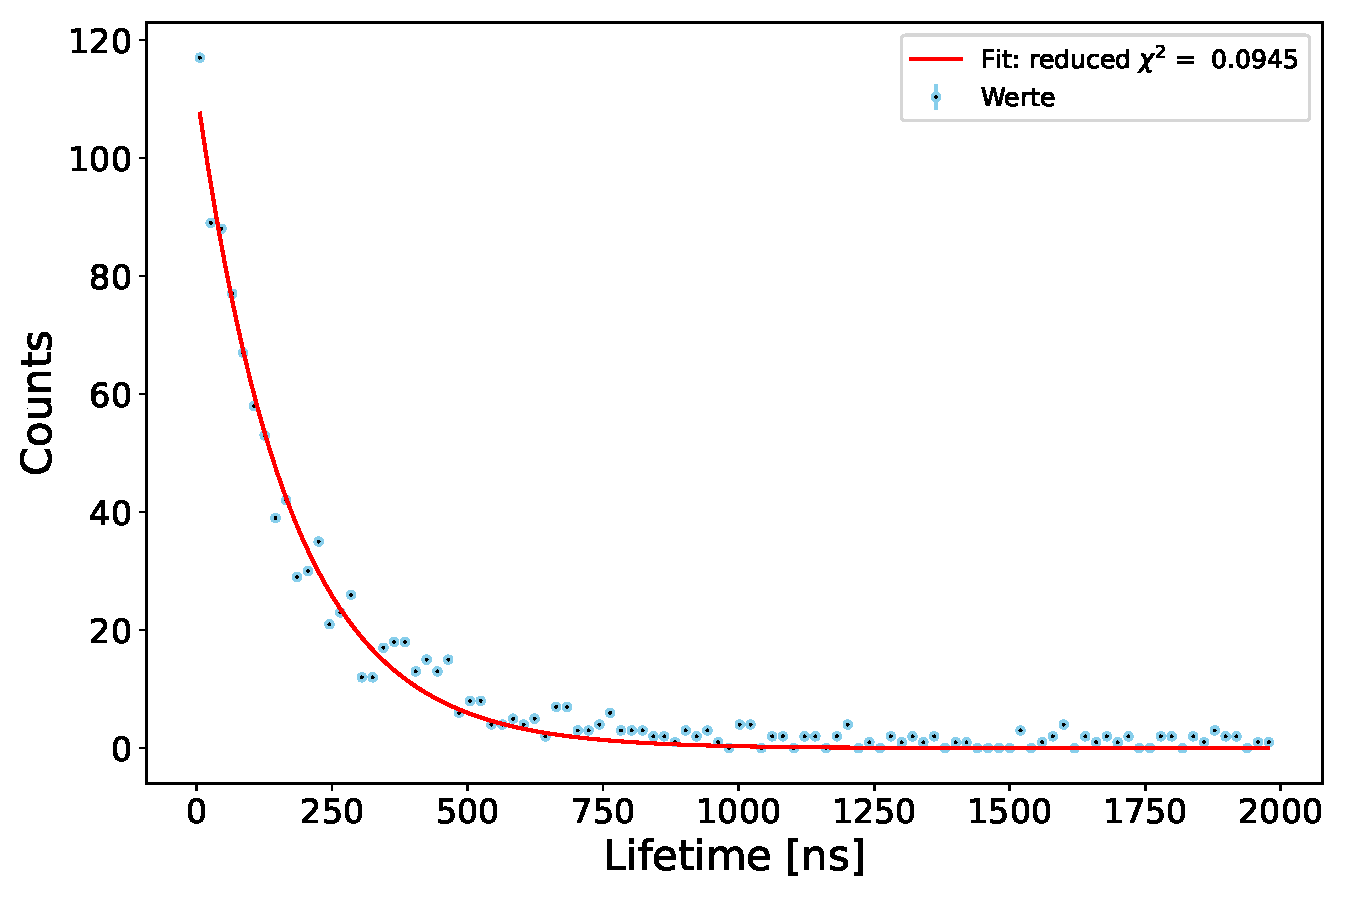
\includegraphics[width= 0.65 \textwidth]{Fits/m13n4_Fit.pdf} 
	\caption{m13n4, Fit} 
 	\label{fig:m13n4, Fit} 
\end{figure}
 \\ 
\begin{table}[ht] 
\centering 
\caption{m13n4, Fit Parameter Tabelle} 
\label{tab:my-table}
\begin{tabular}{|l|c|}
\hline
Parameter Name	&	Wert \\ \hline
amplitude	&	 110.234 \pm  2.136\\ \hline
decay	&	 1.720 \pm  0.0468\\ \hline
\end{tabular} 
\end{table}